%
% File acl2017.tex
%
%% Based on the style files for ACL-2015, with some improvements
%%  taken from the NAACL-2016 style
%% Based on the style files for ACL-2014, which were, in turn,
%% based on ACL-2013, ACL-2012, ACL-2011, ACL-2010, ACL-IJCNLP-2009,
%% EACL-2009, IJCNLP-2008...
%% Based on the style files for EACL 2006 by 
%%e.agirre@ehu.es or Sergi.Balari@uab.es
%% and that of ACL 08 by Joakim Nivre and Noah Smith

\documentclass[11pt,a4paper]{article}
\usepackage[hyperref]{acl2017}
\usepackage{times}
\usepackage{latexsym}
\usepackage[pdftex]{graphicx}

\usepackage{url}

%\aclfinalcopy % Uncomment this line for the final submission
%\def\aclpaperid{***} %  Enter the acl Paper ID here

%\setlength\titlebox{5cm}
% You can expand the titlebox if you need extra space
% to show all the authors. Please do not make the titlebox
% smaller than 5cm (the original size); we will check this
% in the camera-ready version and ask you to change it back.

\newcommand\BibTeX{B{\sc ib}\TeX}

\title{Midterm project report for the Natural Language Understanding Systems course}

\author{Federico Giuggioloni \\
  189662 \\
  {\tt federico.giuggioloni@studenti.unitn.it}}

\date{}

\begin{document}
\maketitle
\begin{abstract}
  This work provides a concept tagging tool for queries related to movies, such as "who is the director of thor".
  The final version of the script enables tweaking of various learning parameters to better evaluate which setting is the best for the situation.
  % TODO Write which version achieves the best F1 score
\end{abstract}

\section{Introduction}

\section{Data set analysis}

% Dataset explanation, similar to README
The dataset is subdivided into a training set and a test set.
These sets are in a word per line format, with the sentences being separated by an empty line.
Multiple columns represent the features of the specific word (such as part-of-speech tag and the lemma) and the correct concept tag.

An analysis of the distribution of the data provided was deemed necessary to ensure it's correct usage.

\subsection{Zipf's law}

The first analysis performed on the training data is to check whether or not Zipf's law is verified.
Due to the nature of the data, a bias towards words typical of the movie industry was expected.
This can be seen clearly in the word frequency distribution, with "movies" and "movie" occupying respectively the second and fifth spot.
(with "movies" appearing more frequently than "of")

%Histogram that shows Zipf's law in action
\begin{figure}[h]
\centering
  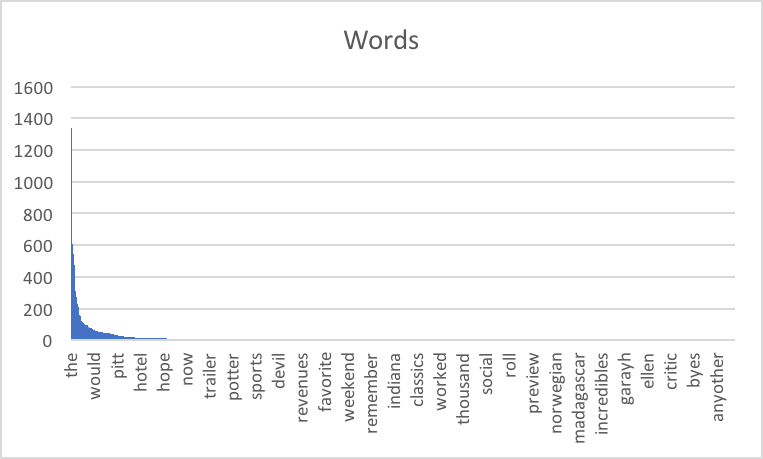
\includegraphics[width=.9\linewidth]{Images/zipf}
  \caption{Zipf's law}
\label{fig:zipf}
\end{figure}


\subsection{Concept distribution}

The most frequent concept is "movie.name" by a wide margin, which means this plus out-of-span tags make up 86\% of the tags present in the training dataset.

%Histogram with concept distribution and generalization distribution
\begin{figure}[h]
\centering
  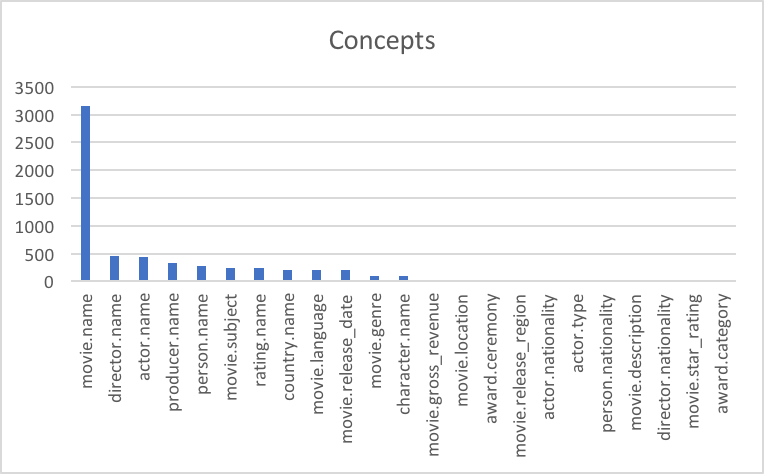
\includegraphics[width=.9\linewidth]{Images/concepts}
  \caption{Concept distribution}
\label{fig:zipf}
\end{figure}

\section{Baseline solution}
The case of a single transducer from word to concept will be taken in consideration as the baseline for all the proposed solutions.
This doesn't take into consideration the structure of the phrase so it is expected to be very inaccurate. 

\begin{verbatim}
accuracy:  67.32%
precision:  20.15%
recall:  54.72%
FB1:  29.45
\end{verbatim}

The resulting F1-Score is very low as expected.

\section{Direct solution}

The simplest and most direct method is obtained by simply composing the transducer from the previous step with the concept model trained on the training data.
To do this the training data was converted from word-per-row to a concept sentence-per-row format. These sentences have been used to train a wide array of language models, by changing the order of the n-grams and the smoothing method.

It can be observed that using a language model trained on bigrams achieves better performance than one trained on trigrams, which can be explained by looking at the training and test sets.
% TODO need to check this A few concept tags only appear as bigrams in the training corpus, while they appear only as trigrams in the test one.

\begin{verbatim}
Smoothing method: witten_bell
Order: 3-grams
Cut-Off: none
accuracy:  92.62%
precision:  76.58%
recall:  74.61%
FB1:  75.58
\end{verbatim}

\begin{verbatim}
Smoothing method: witten_bell
Order: 2-grams
Cut-Off: none
accuracy:  92.68%
precision:  78.51%
recall:  74.34%
FB1:  76.37
\end{verbatim}

\section{Solution using extra features}

The next experiment was to try and include the extra features included in the dataset to improve the F1-Score.
At a first glance the chaining of multiple transducers, each passing from one feature to the next, seemed like a good idea.
Because of this 3 transducers were built and composed: word-to-lemma, lemma-to-part of speech, part of speech-to-concept tag.
By composing the result with the concept model it is shown to be even worse than the baseline:

\begin{verbatim}
Smoothing method: witten_bell
Order: 2-grams
Cut-Off: none
accuracy:  72.81%
precision:  27.35%
recall:   6.14%
FB1:  10.03
\end{verbatim}

An explanation can be found by considering that this method is reducing the input space of the final transducer from the size of the vocabulary to just 38 pos-tags.

Because of this, a second method which keeps the first transducer, while replacing the second and third with a lemma-to-concept transducer.
The second transducer takes into consideration the pos-tags in the calculation of the weights.

\begin{verbatim}
Smoothing method: witten_bell
Order: 3-grams
Cut-Off: none
accuracy:  92.34%
precision:  76.06%
recall:  73.97%
FB1:  75.00
\end{verbatim}

The performance of this method is comparable to the version without extra features.


\section{Solution with generalization}
As the inclusion of the extra features does not seem to improve performance this method does not use them.

The idea was to create two transducers, one that transforms words into a generalization (a word class), while the second transduces from a word class to a concept. The method was implemented by pre-processing the training set, adding a "word class" column created as a derivative of the concept tag. Because of this, including the fact that the only generalization that provides a decent score does nothing more than remove the IOB part of the tags, the performance is lower than the standard method:
\begin{verbatim}
Smoothing method: witten_bell
Order: 3-grams
Cut-Off: none
accuracy:  88.70%
precision:  61.42%
recall:  61.14%
FB1:  61.28
\end{verbatim}

\section{Using frequency cut-off}

Frequency cut-off can be applied to all the previous solutions, but it does nothing to improve the performance.
In fact the resulting concept tagger achieves slightly lower scores when used with a cut-off of 1 (removing words that appear only 1 time in the training corpus):
\begin{verbatim}
Smoothing method: witten_bell
Order: 2-grams
Cut-Off: 1
accuracy:  91.74%
precision:  77.95%
recall:  70.30%
FB1:  73.93
\end{verbatim}

F1 Score of 73.93, almost 2 points lower than the same solution used without cut-off.
The cut-off does remove a lot of the words that are written incorrectly such as "accumalate" and specific movie related terms such as "Dory", which may be desirable when dealing with larger amounts of data.

\section{Pre-processing the training set}

Having the "O" Concept tag assigned to most of the words in the training corpus meant that the concept model would learn that the O tag is very likely in any part of the sentence.
To try and solve this problem, a pre-processing of the training set is done by replacing every \verb|O| tag into a \verb|O-<word> tag|, effectively increasing the total number of concept tags by the number of words.
By doing so, the concept model yields more information regarding the other tags, which are lower in number, and it is possible to achieve a significant improvement on the F1-Score. The following scores have been obtained by using the \textit{no extra features} solution described precedently with the pre-processed training corpus:

\begin{verbatim}
Smoothing method: witten_bell
Order: 3-grams
Cut-Off: none
accuracy:  93.72%
precision:  80.04%
recall:  82.68%
FB1:  81.33
\end{verbatim}

It is interesting to note that using 2-grams with the same smoothing method degrades performance (as opposed to the solution without the pre-processing).

Cut-Off deteriorates performance, so it is still kept at 0.

\begin{verbatim}
Smoothing method: witten_bell
Order: 2-grams
Cut-Off: none
accuracy:  93.13%
precision:  78.35%
recall:  80.29%
FB1:  79.31
\end{verbatim}

The best possible score is obtained by exaggerating on the order of the n-grams at learning time of the concept model(and thus increasing the model's complexity):

\begin{verbatim}
Smoothing method: kneser_ney
Order: 9-grams
Cut-Off: none
accuracy:  94.39%
precision:  82.38%
recall:  83.13%
FB1:  82.76
\end{verbatim}


\section{Conclusions}
The value to be used for the learning parameters depends on the distribution of the data we are using for the learning itself. Just increasing the order of the n-grams used to learn the language model can hurt performance instead of improving it. An example of this is the performance achieved using 2-grams and the witten bell smoothing method, which is higher than the same method used with 3-grams.

Extra features don't improve the concept tagger's score as we would need those features to be available at test time to improve performance. Having only the words themselves at test time means that every single extra feature we want to use to guess the concept tag would have to be estimated from the word itself, increasing the possibility of error.

Minimum frequency cut-off seems to degrade performance for every proposed solution, even though it removes words spelled wrong and some words specific to certain movies.

Finally, the biggest improvement to performance was achieved simply by manipulating the training data in a very specific manner. The analysis of the data used for training and testing is essential to reach the desired accuracy.




\cite{P16-1001}



% include your own bib file like this:
%\bibliographystyle{acl}
%\bibliography{acl2017}
\bibliography{acl2017}
\bibliographystyle{acl_natbib}

\appendix

\end{document}
